\documentclass[mathserif,blue]{beamer}
\usepackage{amssymb}
\usepackage[noindent,space]{ctex}%宏包加载
\usetheme{Boadilla}\beamersetaveragebackground{black!10}%主题设置
\setbeamersize{text margin left=1.3cm}\setbeamersize{text margin right=1.2cm}%页面尺寸
\newcommand\colorwordsa[1]{\textcolor[rgb]{0,.63,.91}{\small\heiti #1}}%彩色文字
\def\threesides{\begin{picture}(14,12)\put(0,0){\qbezier(0,0)(0,8)(7,12)\qbezier(7,12)(14,8)(14,0)\qbezier(14,0)(7,-4)(0,0)}\end{picture}}%logo
\newlength\lengtha\newcommand\an[1][a]{\ensuremath{\{#1_n\}}}\newcommand\lines[1][1.2]{\,\underline{\mbox{\hspace{#1cm}}}\,}% 代码
\setbeamercolor{mycolor}{fg=black,bg=pink}\setbeamercolor{myupcol}{fg=white,bg=purple}\setbeamercolor{mylowcol}{fg=black,bg=pink}% 彩色盒子
\newcommand\beamercolortextbox[1]{\settowidth\lengtha{#1}\hspace{.5em}\raisebox{-.6ex}{\begin{beamercolorbox}[rounded=true,shadow=true,wd=\lengtha,colsep*=-.4ex]{mycolor}#1\end{beamercolorbox}}}
\newcommand\beamercolorlinebox[1]{\settowidth\lengtha{#1}\centerline{\begin{beamercolorbox}[rounded=true,shadow=true,wd=\lengtha]{mycolor}#1\end{beamercolorbox}}}
\begin{document}

\title{等比数列}
\author{王崇宁}
\institute[西大]{西南大学}
\logo{\threesides}
\maketitle


\begin{frame}{引入}
\begin{columns}
\begin{column}{0.55\textwidth}
  \fbox{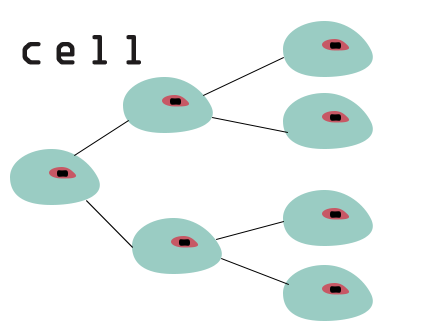
\includegraphics[width=0.8\textwidth]{cell.png}}\par\vspace{1.5ex}\fbox{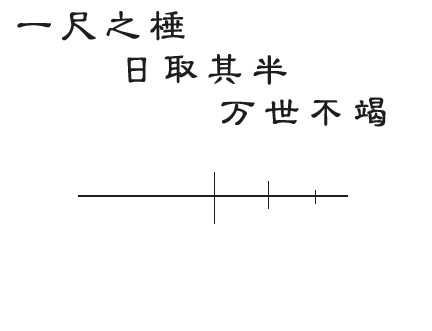
\includegraphics[width=0.8\textwidth]{frac.png}}
\end{column}\pause
\begin{column}{0.45\textwidth}
  \begin{beamerboxesrounded}[shadow=ture]{第一个数列}
  $1,~2,~4,~8,~16,~32,\cdots$
  \end{beamerboxesrounded}\par\vspace{.8in}\pause
  \begin{beamerboxesrounded}[shadow=ture]{第二个数列}
  $1,~\dfrac12,~\dfrac14,~\dfrac18,~\dfrac1{16},~\dfrac1{32}\cdots$
  \end{beamerboxesrounded}
  \end{column}
\end{columns}
\end{frame}


\begin{frame}{你会类比吗}
\kaishu
  \begin{columns}
  \begin{column}{0.5\textwidth}
    \begin{block}<1->{等差数列}
      如果一个数列\an 从第 2 项起, 每一项与它前一项的\textbf{差}都等于同一个常数, $$a_{n}-a_{n-1}=d~~(n\geqslant2)$$ 这样的数列叫做\colorwordsa{等差数列}, 这个常数$d$ 叫做等差数列的\colorwordsa{公差}.
    \end{block}
  \end{column}
  \begin{column}{0.5\textwidth}
    \begin{block}<2>{等比数列}
      如果一个数列\an 从第 2 项起, 每一项与它前一项的\textbf{比}都等于同一个常数, 即$$\frac{a_{n}}{a_{n-1}}=q~~(n\geqslant2)$$这样的数列叫做\colorwordsa{等比数列}, 这个常数$q$叫做等比数列的\colorwordsa{公比}.
    \end{block}
  \end{column}
  \end{columns}
\end{frame}


\begin{frame}{存在的,不一定是合理的}
  \begin{exampleblock}{例1:下列数列是不是等比数列, 若是,说出公比}
  %\setbeamercovered{transparent}
  \begin{enumerate}
    \item $2,~2,~2,~2,~2,~2$;\pause\hspace*{\fill}$q=1$\hspace*{.5in}\pause
    \item $2^{-1},~2^1,~2^3,~2^5,~2^7,~2^9$;\pause\hspace*{\fill}$q=4$\hspace*{.5in}\pause
    \item $-1,~10,~-10^2,~10^3,~-10^4,~10^5$;\vspace{1ex}\pause\hspace*{\fill}$q=-10$\hspace*{.5in}\pause
    \item $\alt<7>{0,~}{}-1,~-\dfrac12,~-\dfrac14,~-\dfrac18,~-\dfrac1{16}$;\vspace{1ex}\pause\pause\hspace*{\fill}$ q=\dfrac12$\hspace*{.5in}\pause
    \item $~a^1,~a^2,~a^3,\cdots,~a^n,\cdots$\alt<10>{;}{$(a\ne0)$;}\pause\pause\hspace*{\fill}$q=a$\hspace*{.5in}\pause
  \end{enumerate}
  \end{exampleblock}
  \begin{alertblock}{注意}\pause
    \begin{itemize}[<+->]
       \item 等比数列\an 中, 每一项$a_n$与公比$q$都不等于\alert{$0$};
       \item 等比数列的奇数项同号,偶数项也同号.
     \end{itemize}
  \end{alertblock}
\end{frame}


\begin{frame}{等比数列的判定}
  \begin{exampleblock}{例2}
    已知数列\an 的前$n$项和$S_n=3a_n+1$,求证:\an 是等比数列.
  \end{exampleblock}\pause
  \begin{block}{解:}\pause
    由 $a_1=S_1=3a_1+1$, 得 $ a_1=-\dfrac12\neq0$, \\\pause
    当 $n\geqslant2\text{时},~ a_{n}=S_{n}-S_{n-1}=3a_{n}+1-(3a_{n-1}+1)$\\
      \hspace{8em}$=3a_{n}-3a_{n-1}$;\\
      \pause\vspace{1ex}
      所以 $a_{n}=\dfrac32a_{n-1},$\\\pause\vspace{1ex}
      又因为 $a_1\ne0$, 所以 \an 是等比数列.
  \end{block}
\end{frame}


\begin{frame}{等比中项}
\vspace*{-0.8in}
  \begin{block}{定义}\kaishu
    与等差中项的概念类似, 如果数列$a, b, c$成等比数列, 那么$b$叫做$a$与$c$的\colorwordsa{等比中项}.
  \end{block}
  \begin{itemize}
    \item<3-> $b$是$a,c$的等比中项的等价于\alt<3>{\beamercolortextbox{$b^2=ac~\text{且}~b\ne0$}}{$b^2=ac~\text{且}~b\ne0$}
    \item<4-> 在数列\an 中, 若\beamercolortextbox{$a_{n-1}a_{n+1}=a_n^2~\text{且}~a_n\ne0~(n\geqslant2)$} 则\an 是等比数列.
  \end{itemize}\pause\vspace*{-2.7in}
  \qquad
\includegraphics[width=0.4\textwidth]{double.png}\qquad
\includegraphics[width=0.4\textwidth]{doublee.png}
\end{frame}


\begin{frame}{}
  \begin{exampleblock}{例3}
    若等比数列\an 中, $a_3=3,\ a_5=5,$求$a_4$.
  \end{exampleblock}
    \pause
  \begin{block}{解:}
    由$a_4$为$a_3,\,a_5$的等比中项, 得
    $$a_4^2=a_3a_5=15.$$\pause
    所以$a_4=\pm\sqrt{15}$.
  \end{block}
\end{frame}


\begin{frame}{易错点}
  \begin{exampleblock}{例4}
    若等比数列\an 中, $a_1=3,\ a_5=12,$求$a_3$.
  \end{exampleblock}\pause
  \begin{block}{解:}
    因为$a_1,a_3,a_5$成等比数列, 所以$a_3^2=a_1a_5=36$,\\
    因此$a_3=\pm6$.\\\pause
    又因为$a_1>0$, 所以$a_3=6$.
  \end{block}
    \pause\vspace{1ex}
  \begin{beamerboxesrounded}[upper=myupcol,lower=mylowcol,shadow=true]{注意}
    等比数列奇数(或偶数)位上的符号总相同.
  \end{beamerboxesrounded}\vspace{9pt}
\end{frame}


\begin{frame}{又一道题}
\begin{exampleblock}{例5}
    已知等比数列\an 的前 3 项分别为$\sqrt2,~\sqrt[3]2,~\sqrt[6]2$%$\Dd2^{\frac12},2^{\frac13},2^{\frac16}$,
    则该数列的第 4 项为\alt<1>{\lines}{\lines\hspace{-2em}$1$}\pause
  \end{exampleblock}\pause
  \begin{block}{解}
  法 1 (等比中项):~$a_4\cdot\sqrt[3]2=(\sqrt[6]2)^2=\sqrt[3]2,~~\therefore~a_4=1$.\\\vspace{1ex}\pause
  法 2 (求公比):~$q=\dfrac{2^{1/3}}{2^{1/2}}=2^{-1/6}$,\\\vspace{1ex}
  $\therefore~a_4=a_3q=2^{1/6}2^{-1/6}=1.$
  \end{block}
\end{frame}


\begin{frame}{通项公式}
\begin{exampleblock}{问题}
  设等比数列\an 的首项为$a_1$, 公比为$q$, 求\an 的通项公式.
  \end{exampleblock}
    \pause
  \begin{block}{推导}
  因为$a_n=\dfrac{a_n}{a_{n-1}}\dfrac{a_{n-1}}{a_{n-2}}\cdots\dfrac{a_2}{a_1}a_1=a_1q^{n-1}$\par
  \setbeamercolor{myupcol}{fg=white,bg=brown}
  \end{block}
    \pause
  \begin{alertblock}{结论}
  \setbeamercolor{mylowcol}{fg=black,bg=pink}
  所以\an 的通项公式为\hspace{.5em}\beamercolorlinebox{$a_n=a_1q^{n-1}$}
  \end{alertblock}
\end{frame}


\begin{frame}{这不是最后一道题}
  \begin{exampleblock}{例6}
    已知等比数列\an 中, \\
    (1)$a_4=2,a_7=8$, 求$a_n$;\\
    (2)$a_2+a_5=18$, $a_3+a_6=9$, $a_n=1$, 求$n$.
  \end{exampleblock}\pause
  \begin{block}{解:}\pause
  \begin{columns}
    \begin{column}{0.45\textwidth}
      (1)设\an 的公比为$q$,则\vspace*{-2ex}
    \begin{equation*}
      \begin{cases}
        a_1q^3&=2\\
        a_1q^6&=8
      \end{cases}
    \end{equation*}\vspace*{-2ex} \par\pause
        解出$q=\sqrt[3]{4}$,$a_1=\frac12$.\\\pause
        所以$a_n=a_1q^{n-1}=2^{\tfrac{2n-5}{3}}$.\\\pause
    \end{column}
    \begin{column}{0.45\textwidth}
        (2)设\an 的公比为$q$,则\vspace*{-2ex}
      \begin{equation*}
        \begin{cases}
          a_1q+a_1q^4&=18\\
          a_1q^2+a_1q^5&=9
        \end{cases}
      \end{equation*}\vspace*{-2ex} \par\pause
        解出$q=1/2$,$a_1=32$.\\\pause
        所以$a_n=a_1q^{n-1}=2^{6-n}$.\\\pause
        令$a_n=1$, 得$n=6$.
    \end{column}
  \end{columns}
  \end{block}
\end{frame}

\newcommand{\liness}{\raisebox{-0.2em}{\lines}}
\begin{frame}{等比数列的一些性质}
  性质1:$a_n=a_m\cdot q^{n-m}\quad(m,n\in\mathbf{N^*})$\\
  性质2:若$m+n=l+k~(m,n,l,k\in\mathbf{N^*})$, 则$a_m\cdot a_n=a_l\cdot a_k$.\pause
  \begin{exampleblock}{例7:小题轰炸}
    在等比数列\an 中, \\
    (1)$\text{若}a_5=27,~q=3,\text{则}~a_1=$\alt<1,2>{\liness}{\liness\hspace{-1cm}$3^{-1}$}\\\vspace{1ex}
    (2)$\text{若}a_4a_8=16,\text{则}~a_5a_6a_7=\alt<1,2,3>{\liness}{\liness\hspace{-1cm}\pm64}$\\\vspace{1ex}
    (3)$\text{若}a_3a_5=4,\text{则}~a_2a_4a_6=\alt<1,2,3,4>{\liness}{\liness\hspace{-1cm}\pm8}$\\\vspace{1ex}
    (4)$\text{若}a_1+a_5=5,~a_2a_4=6,\text{则}~a_9=$\alt<1,2,3,4,5>{\liness}{\liness\hspace{-1.2cm}\raisebox{.3em}{$\dfrac92\text{或}\dfrac43$}}\\\vspace{1ex}
  \end{exampleblock}\pause\pause\pause\pause
\end{frame}

\begin{frame}{小结}
\setbeamercovered{transparent}
\begin{itemize}[<+->]\pause
  \item 数列\an 为等比数列的定义是$\dfrac{a_n}{a_{n-1}}=q~(n\geqslant2)$, 或者$a_{n}=a_{n-1}q, (n\geqslant2,a_1,q\neq0)$.
  \item 等比数列的各项非零, 而且奇(偶)数项的符号相同.
  \item $a,b,c$成等比数列$\Leftrightarrow b$是$a,c$的等比中项$\Leftrightarrow b^2=ac,~b\neq0 $
  \item 等比数列\an 的通项公式为$a_n=a_1q^{n-1}$.
  \item $a_n=a_mq^{n-m}~(m,n\in\mathbf{N^*})$; \\若$m+n=l+k~$, 则$a_ma_n=a_la_k$ $(m,n,l,k\in\mathbf{N^*})$.
\end{itemize}
\end{frame}

\end{document}

